\section{Impact}
\begin{frame}[c]{Derivative Works of PointNet}
    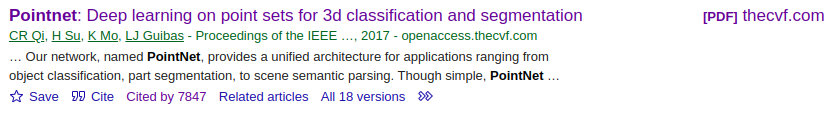
\includegraphics[width=\textwidth]{impact}
    \large
    \pause
    Core architecture ideas were adapted in:
    \begin{multicols}{2}
        \begin{itemize}
            \item A sift-like network module \cite{jiang2018sift}
            \item Similarity group proposal network \cite{wang2018sgpn}
            \item Point cloud upsampling \cite{yu2018pu}
            \item Application to Neuroanatomy \cite{gutierrez2018deep}
            \item Frustum pointnets \cite{qi2018frustum}
            \item Pointcnn \cite{li2018pointcnn}
            \item many more ...
        \end{itemize}
    \end{multicols}
    \pnote{
        Auswirkungen von PointNet erstmal nicht wenig \\
        Anfang schreiben: ~7300 \\
        Immernoch höchst relevant
    }
\end{frame}

\begin{frame}[c]{Derivative Works of PointNet II}
    \large
    \begin{multicols}{2}
        PointNet has been used as a module in:
        \begin{itemize}
            \item PointNet++~\cite{qi2017pointnet++}
            \item SyncSpecCNN~\cite{yi2017syncspeccnn}
            \item VoxelNet~\cite{zhou2018voxelnet}
            \item ...
        \end{itemize}
        \begin{figure}
            % 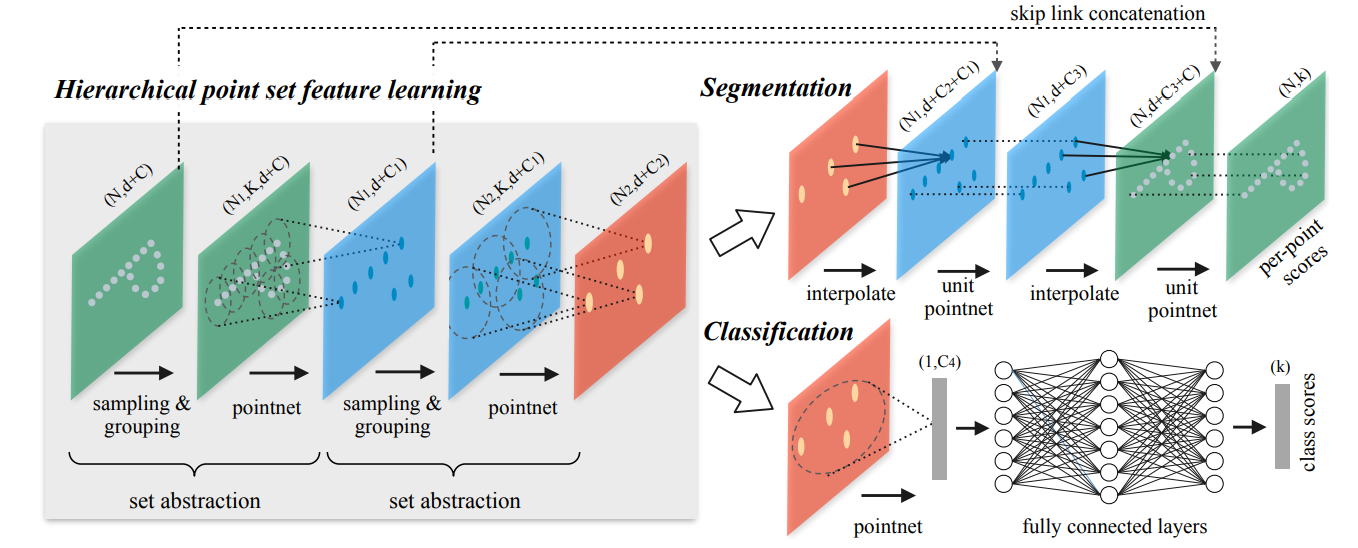
\includegraphics[width=0.5\textwidth]{pointnet_plusplus}
            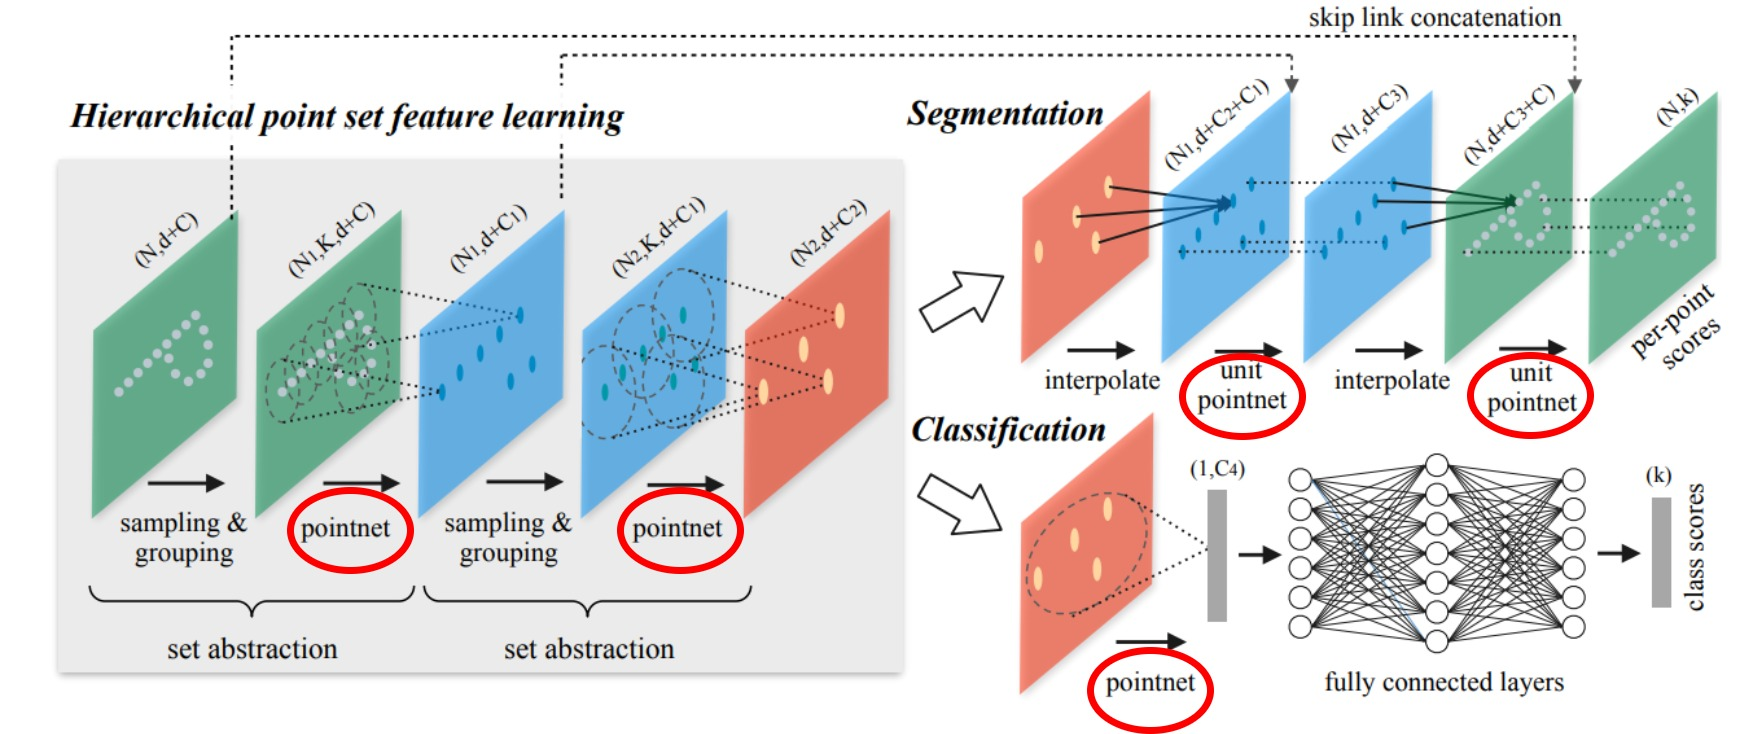
\includegraphics[width=0.5\textwidth]{pointnet++_architecture}
            \caption{Architecture of PointNet++ with highlighted PointNet layers. Figure adapted from PointNet++~\cite{qi2017pointnet++}}
        \end{figure}
    \end{multicols}
    \pnote{
        Was auch passiert ist, ist dass es als modul / layer  \\
        verwendet wird
    }
\end{frame}

